\documentclass[14pt,fleqn]{extarticle}
\RequirePackage{prepwell}
\previewoff
\begin{document}

\newcommand\tri{\triangle ABC}
\newcommand\ab{ \left(\frac{5}{2}x - 9 \right)}
\newcommand\bc{ \left(-x+12 \right)}
\newcommand\ca{ \left(\frac{3}{4}x - 2 \right)}

%text
Using integration, find the area of the 
$\triangle ABC$ whose vertices are 
\[ \quad A = (4,1), B = (6,6) \text{ and } C = (8,4) \]
%
 
\newcard 

The points $A,B$ and $C$ are as shown in the figure below. This gives us the following triangle 

\begin{center} 
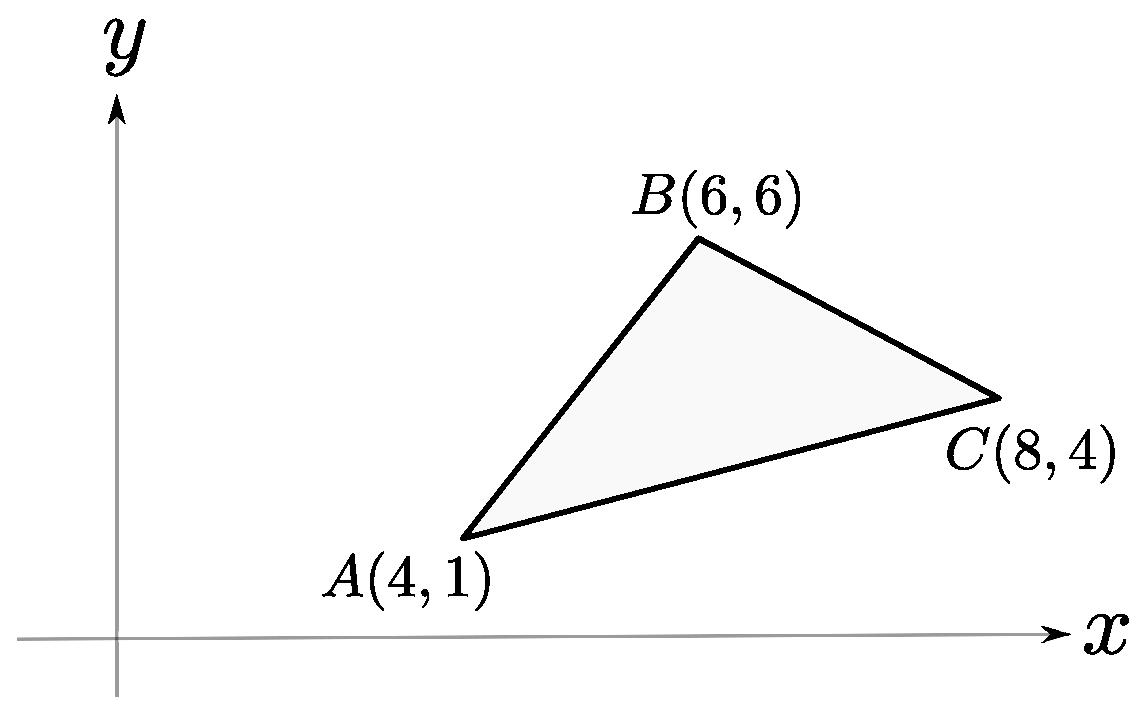
\includegraphics[scale=0.35]{figure.eps} 
\end{center} 

\newcard

The equations of the sides of $\tri$ are

\begin{center}
\begin{tabular}{NN}
\midrule 
\text{Side} & \text{Equation} \\
\midrule
AB & y=\frac{5}{2}x-9 \\ 
\midrule 
BC & y=-x+12 \\
\midrule 
CA & y= \frac{3}{4}x -2 \\
\midrule 
\end{tabular}
\end{center} 

\newcard 
The equations of the sides of $\tri$ are

\begin{center}
\begin{tabular}{NN}
\midrule 
\text{Side} & \text{Equation} \\
\midrule
AB & y=\frac{5}{2}x+7 \\ 
\midrule 
BC & y=x+12 \\
\midrule 
CA & y= -\frac{3}{4}x + 2 \\
\midrule 
\end{tabular}
\end{center} 

\newcard

Apply the two-point formula to find the 
equations of the sides. 
%
\begin{align}
AB: \frac{y-1}{x-4} &= \frac{6-1}{6-4} = \frac{5}{2} \\
\implies 2y-2 &= 5x-20\implies y = \frac{5}{2}x -9 \\
BC:\frac{y-6}{x-6} &= \frac{4-6}{8-6} = -1 \\ 
\implies y-6 &= -x + 6 \implies y = -x + 12 \\
CA: \frac{y-1}{x-4} &= \frac{4-1}{8-4} = \frac{3}{4} \\
\implies 4y-4 &= 3x-12 \implies y=\frac{3}{4}x -2 
\end{align}
%
\newcard 

The expression for the required area $R$ is therefore 

\begin{align}
	R &= \int_4^6 \ab\cdot dx + \int_6^8 \bc\cdot dx \\
	&- \int_4^8 \ca \cdot dx 
\end{align}

\newcard

The expression for the required area $R$ is therefore 

\begin{align}
	R &= \int_4^6 \ab\cdot dx + \int_6^8 \bc\cdot dx 
\end{align}


\newcard

%text
From the figure, we can see that the 
required area is as follows 

%
\begin{align}
\therefore R &= \underbrace{\int_4^6\left( \frac{5x}{2}-9\right)\cdot dx}_{\text{Area under AB}} 
+ \underbrace{\int_6^8(-x+12)\cdot dx}_{\text{Area under BC}} \\
&- \underbrace{\int_4^8\left( \frac{3x}{4}-2\right)\cdot dx}_{\text{Area under CA}}
\end{align}

\newcard

\begin{align}
	R &= \overbrace{\int_4^6 \ab\cdot dx}^{= 7} + \overbrace{\int_6^8 \bc\cdot dx}^{=10} \\
	&- \underbrace{\int_4,8 \ca\cdot dx}_{=10} \\
	&= 7\text{ sq. units} 
\end{align}

\newcard 

\begin{align}
	R &= \overbrace{\int_4^6 \ab\cdot dx}^{= 8} + \overbrace{\int_6^8 \bc\cdot dx}^{=11} \\
	&- \underbrace{\int_4,8 \ca\cdot dx}_{=10} \\
	&= 9\text{ sq. units} 
\end{align}


\newcard 

\begin{align}
X &= \int_4^6\left(\frac{5x}{2}-9\right)\cdot dx  
=\left[ \frac{5x^2}{4}-9x \right]_4^6 \\
&= \left[ \left(45-54\right)-\left(20-36\right) \right] =  7 \\
Y &= \int_6^8(-x+12)\cdot dx = \left[-\frac{x^2}{2}+12x \right]_6^8 \\
&=  \left[ \left(-32+96\right)-\left(-18+72\right) \right] =10 \\
Z &= \int_4^8\left( \frac{3x}{4}-2\right)\cdot dx = \left[ \frac{3x^2}{8}-2x\right]_4^8 \\
&=  \left[ \left(24 -16\right)-\left(6-8\right) \right] = 10 \\
\therefore R &= X+Y-Z = 7\text{ sq. units}
\end{align}

\end{document}